%%%%%%%%%%%%%%%%%%%%%%% file template.tex %%%%%%%%%%%%%%%%%%%%%%%%%
%
% This is a template file for The European Physical Journal
%
% Copy it to a new file with a new name and use it as the basis
% for your article
%
%%%%%%%%%%%%%%%%%%%%%%%% Springer-Verlag %%%%%%%%%%%%%%%%%%%%%%%%%%
%
% \begin{filecontents}{leer.eps}
%!PS-Adobe-2.0 EPSF-2.0
%%CreationDate: Mon Jul 13 16:51:17 1992
%%DocumentFonts: (atend)
%%Pages: 0 1
%%BoundingBox: 72 31 601 342
%%EndComments

% gsave
% 72 31 moveto
% 72 342 lineto
% 601 342 lineto
% 601 31 lineto
% 72 31 lineto
% showpage
% grestore
%%Trailer
%%DocumentFonts: Helvetica
% \end{filecontents}
%
\documentclass[epj, nopacs]{svjour}
% Remove option referee for final version
%
% Remove any % below to load the required packages
%\usepackage{latexsym}
\usepackage{graphics}
\usepackage[
    locale=US,
    separate-uncertainty=true,
    per-mode=fraction,    
    print-unity-mantissa = false,
]{siunitx}
\DeclareSIUnit\clight{\text{\ensuremath{c}}}
\sisetup{math-micro=\text{µ},text-micro=µ}
\usepackage{amsmath}
\usepackage{float}
\usepackage{scrhack}
\floatplacement{figure}{htbp}
\floatplacement{table}{htbp}
\usepackage{hyperref}
\usepackage[
backend=biber,
style=numeric,
sorting=none,
natbib
]{biblatex}
\addbibresource{lit.bib}
\usepackage{microtype}
\usepackage{booktabs}


\hyphenation{pa-ra-me-tri-zed}
\hyphenation{Brems-strah-lung}
%
\begin{document}
%
\title{Simulation of Deflection Uncertainties on Directional Reconstructions of Muons Using PROPOSAL}
% \subtitle{Do you have a subtitle?\\ If so, write it here}
\author{Pascal Gutjahr\inst{1}\fnmsep\thanks{\email{pascal.gutjahr@udo.edu} (corresponding author)} \and Jean-Marco Alameddine\inst{1} \and Alexander Sandrock\inst{2} \and Jan Soedingrekso\inst{1} \and Mirco Hünnefeld\inst{1} \and Wolfgang Rhode\inst{1}  
}
%
\institute{Department of Physics, TU Dortmund University, Otto-Hahn-Straße~4, Dortmund 44227, Germany \and 
          Faculty of Mathematics and Natural Sciences, University of Wuppertal, Gaußstraße~20, Wuppertal 42119, Germany}
%
\date{Received: date / Revised version: date}
% The correct dates will be entered by Springer
%
\abstract{
  Large scale neutrino detectors and muon tomography rely on the muon direction in the detector to infer the muon's or parent neutrino's origin. However, muons accumulate deflections along their propagation path prior to entering the detector, which may need to be accounted for as an additional source of uncertainty. 
  In this paper, the deflection of muons is studied with the simulation tool PROPOSAL, which accounts for multiple scattering and deflection on stochastic interactions. Deflections along individual interactions depend on the muon energy and the interaction type and can reach up to the order of degrees -- even at TeV to PeV energies. The accumulated deflection angle can be parametrized in dependence of the final muon energy, independent of the initial muon energy. The median accumulated deflection of a propagated muon with a final energy of $\SI{500}{\giga\electronvolt}$ is $\theta_{\text{acc}} = 0.10_{-0.02}^{+0.27}\,\si{\degree}$ 
  with a $\SI{95}{\percent}$ central interval. This is on the order of magnitude of the directional resolution of present neutrino detectors. Furthermore, comparisons with the simulation tools MUSIC and Geant4 as well as two different muon deflection measurements are performed.
  \keywords{Neutrino Astronomy -- Neutrino Source Search -- Angular Resolution -- Muon Tomography}
%
\PACS{
      {PACS-key}{discribing text of that key}   \and
      {PACS-key}{discribing text of that key}
     } % end of PACS codes
} %end of abstract
%

\maketitle
%
\section{Introduction}\label{sec:introduction}

The directional reconstruction of muons is an essential task for muon tomography or large scale neutrino detectors such as IceCube 
\cite{IceCube_Instrumentation} or KM3NeT \cite{KM3NeT_Design}. In both cases, the muon direction is measured at its crossing through the instrumented volume, which is then utilized to infer its origin or the origin of the parent neutrino. 
However, muons may propagate many kilometers prior to entering the detector while interacting with the surrounding medium. 
Along their propagation, muons can undergo many of thousands 
of interactions, depending on their energy and propagation distance. 
These interactions can lead to a deflection of the muon that may need to be accounted for as an additional source of uncertainty in these measurements. 
Current angular resolutions are above
$\SI{0.1}{\degree}$ for  
$\si{\tera\electronvolt}$ to $\si{\peta\electronvolt}$ energies in IceCube 
\cite{IceCube_Resolution2021} 
and below 
$\SI{0.2}{\degree}$ for energies greater than $\SI{10}{\tera\electronvolt}$ in 
KM3NeT \cite{KM3NeT_Resolution2021}.

To study the impact of the muon deflection on the angular resolution 
of current neutrino detectors, 
the paper is structured as follows: in section~\ref{sec:proposal},
the lepton propagator PROPOSAL is briefly described. In section~\ref{sec:defl_per_int},
PROPOSAL \cite{koehne2013proposal, dunsch_2018_proposal_improvements} is used to study the muon deflection per interaction.
The accumulated deflection is analyzed and compared to the propagation codes
MUSIC \cite{MUSIC} and Geant4 \cite{GEANT4} and two measured data in section~\ref{sec:accum_defl}. The findings of this study
are summarized in section~\ref{sec:conclusion}.

\section{Overview of the Simulation Tool PROPOSAL}\label{sec:proposal}

The tool PROPOSAL \cite{koehne2013proposal, dunsch_2018_proposal_improvements} propagates charged leptons and photons through media and is 
used in this paper to simulate the deflection of muons. For this purpose, 
muons are propagated through the media ice and water 
to estimate the deflection for neutrino telescopes such as IceCube and KM3NeT. All relevant muon interaction types 
as bremsstrahlung \cite{KKP_1995, Bremsstrahlung_KKP}, photonuclear interaction \cite{Abramowicz_1997} with 
shadowing \cite{ButkevichMikheyev_2002}, electron pair production \cite{epair_kokoulin_petrukhin} with corrections for the 
interaction with atomic electrons \cite{epair_kelner}, 
ionization described by the Bethe-Bloch formula with corrections for muons \cite{Rossi} 
and the decay are provided by PROPOSAL. The interaction processes are sampled by their cross section.
Since interactions 
with the massless photon as secondary particle can be arbitrarily small, an energy cut is introduced to avoid an infinite number of bremsstrahlung interactions 
and furthermore to increase the runtime performance. 
The cut is applied with a minimum energy loss
\begin{equation}
    E_{\text{loss,min}} = \min{(e_{\mathrm{cut}}, E \cdot v_{\mathrm{cut}})}\,,
\end{equation}
using two parameters -- a total and a relative energy cut denoted as 
$e_{\mathrm{cut}}$ and $v_{\mathrm{cut}}$ with the energy $E$ of the particle 
directly before the interaction. 
By the introduction of 
this energy cut, the next significant energy loss with 
$E_{\mathrm{loss}} \geq E_{\text{loss,min}}$ 
is treated as a stochastic energy loss in the propagation. 
All energy losses with $E_{\mathrm{loss}} < E_{\text{loss,min}}$ between 
two stochastic losses are accumulated and lost continuously, denoted 
as continuous energy loss.
The methodical uncertainties are small 
for a relative energy cut $v_{\mathrm{cut}}\ll 1$, which increases the runtime.
The 
propagation process is defined by an initial muon energy $E_{\text{i}}$ and 
two stopping criteria -- a final energy $E_{\text{f,\,min}}$ and a 
maximum propagation distance $d_{\text{max}}$. If the last interaction of 
a propagation is sampled by a stochastic interaction, the true final energy 
$E_{\text{f}}$ can become lower and the 
propagation distance $d$ can be higher than the required limits. 
Since muons are unstable, a decay leads to a premature 
stop, which is negligible for high energies \cite{phd_soedingrekso}.

The deflections for stochastic interactions are parametrized by Van Ginneken 
in Ref.~\cite{Van_Ginneken} with a direct calculation of the deflection in 
ionization using four-momentum conservation. 
Furthermore, there are parametrizations for stochastic deflections given in Geant4 \cite{GEANT4} 
for bremsstrahlung and photonuclear interaction, which 
are also available in PROPOSAL.
To estimate the deflection along 
a continuous energy loss, multiple scattering described by Molière 
\cite{moliere_scattering} and the Gaussian approximation by Highland 
can be chosen \cite{HIGHLAND_1975}. 
The orientation of the deflection in the plane perpendicular to the muon direction is 
sampled uniformly between $0$ and $2\mathrm{\pi}$.
The latest updates with a detailed description of the whole tool can be found 
in Ref.~\cite{phd_soedingrekso}. 
The stochastic deflections have been implemented in PROPOSAL recently and they are 
described and studied in Ref.~\cite{Gutjahr_2021}.
A publication describing the 
updates in PROPOSAL is in preparation as Alameddine et al.
All simulations are done with PROPOSAL $7.3.1$.

\section{Muon Deflection per Interaction}\label{sec:defl_per_int}
First, the stochastic deflections described by Van Ginneken~\cite{Van_Ginneken} 
and implemented 
in PROPOSAL are investigated in combination with the two multiple scattering methods. 
For this purpose, $\num{1000}$ muons are propagated from $E_{\text{i}} = \SI{1}{\peta\electronvolt}$ to $E_{\text{f,\,min}} = \SI{1}{\tera\electronvolt}$.
The deflections per interaction are presented 
for each interaction type and the sum over all types in Figure~\ref{fig:defl_per_int}. 
The size of individual deflections 
extend over several orders of magnitude with a median of $\SI{3.9e-6}{\degree}$
and a $\SI{95}{\percent}$ central interval of $[\SI{2.2e-7}{\degree}, \,\SI{1.3e-3}{\degree}]$. 
It follows that the deflections are primarily dominated by multiple scattering, except for a few outliers caused by bremsstrahlung, which 
allows very large energy losses and thus the largest deflections. 
The largest median deflection with the highest $\SI{95}{\percent}$ interval results due to photonuclear interaction.
The median propagation distance with the lower and upper $\SI{95}{\percent}$ 
central interval results to $16.4_{-7.3}^{+24.6}\,\si{\kilo\meter}$.
Detailed values for each interaction type can be found in Table~\ref{tab:defl_per_int}.

\begin{figure*}
    \centering 
    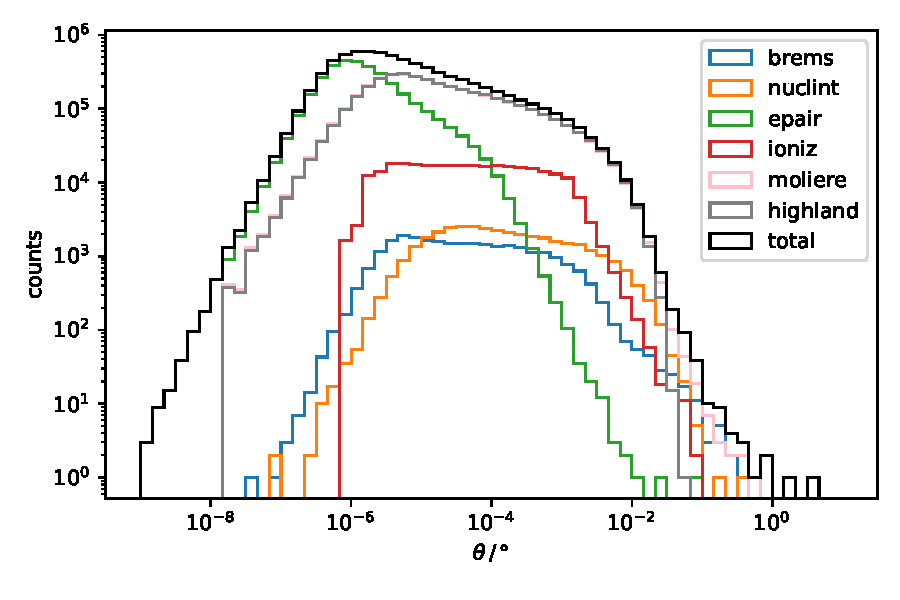
\includegraphics{../../deflection/plots/FINAL/1PeV_1TeV_1000events_deflection_along_sampling.pdf}
    \caption{The muon deflection $\theta$ per interaction in degree is shown for different mechanisms. The propagation is done for $\num{1000}$ 
    muons from $E_{\text{i}} = \SI{1}{\peta\electronvolt}$ to $E_{\text{f,\,min}} = \SI{1}{\tera\electronvolt}$ using $e_{\mathrm{cut}} = \SI{500}{\mega\electronvolt}$ and $v_{\mathrm{cut}} = 0.05$ in ice. 
    The stochastic interactions 
    are stated as Bremsstrahlung (Brems), photonuclear interaction (Nuclint), electron pair produciton (Epair) and ionization (Ioniz).
    Two simulations 
    are done to check both multiple scattering methods Molière and Highland.  
    The total distribution is presented only for all stochastic processes including Molière's. Multiple scattering dominates the deflection. Details are presented in 
    Table~\ref{tab:defl_per_int}.}
    \label{fig:defl_per_int}
\end{figure*}

\begin{table*}
    \centering 
    \caption{The medians of deflections $\theta$ per interaction from Figure~\ref{fig:defl_per_int} are presented for each stochastic interaction type, the two multiple scattering methods and the total distribution including Molière with the upper and lower limits of the $\SI{95}{\percent}$ 
    central intervals. The largest median deflection is caused by photonuclear interaction.}
    \begin{tabular}{ccccccc}
        \toprule 
        Brems & Nuclint & Epair & Ioniz & Molière & Highland & Total  \vspace{6pt} \\
        $\theta\,/\,\SI{e-5}{\degree}$ & $\theta\,/\,\SI{e-5}{\degree}$ & $\theta\,/\,\SI{e-5}{\degree}$ & $\theta\,/\,\SI{e-5}{\degree}$ & $\theta\,/\,\SI{e-5}{\degree}$ & $\theta\,/\,\SI{e-5}{\degree}$ & $\theta\,/\,\SI{e-5}{\degree}$\\
        \midrule 
        $3.8_{-0.1}^{+297}$ & $11.7_{-4.2}^{+963}$ & $0.1_{-0.02}^{+4.2}$ & $4.4_{-0.1}^{+181}$& $1.2_{-0.05}^{+222}$ & $1.2_{-0.05}^{+225}$ & $0.4_{-0.02}^{+129}$\\ 
        \bottomrule
    \end{tabular}
    \label{tab:defl_per_int}
\end{table*}

\section{Accumulated Muon Deflection}\label{sec:accum_defl}

As shown in Section~\ref{sec:defl_per_int}, the deflection per interaction 
is lower than $\sim\SI{1}{\degree}$ in general. Since these deflections accumulate along the 
propagation path, the angle between the incoming and the outgoing 
muon direction is analyzed. This angle limits the angular resolution 
for neutrino source searches utilizing incoming muons, since there is no information 
about the muon before the detector entry.

First, the deflections in PROPOSAL are compared to 
the tools MUSIC \cite{MUSIC,comparison_MUSIC_GEANT4_2009} and Geant4 \cite{GEANT4}.
MUSIC (MUon SImulation Code) is a tool to simulate the propagation of muons 
through media like rock and water considering the same energy losses as in 
PROPOSAL. Also, the losses are divided into continuous and stochastic 
energy losses by a relative energy cut. Several cross sections, multiple scattering 
methods and parametrizations for stochastic deflections are 
available. For these studies, the same cross section parametrizations 
as in PROPOSAL are chosen, except those for 
photonuclear interaction \cite{nulcint_bugaev_Shlepin, bugaev_1980_defl,bugaev_1981_defl}. The stochastic deflections are also parametrized by 
Van Ginneken~\cite{Van_Ginneken}. 
The Gaussian 
approximation \cite{HIGHLAND_1975} is set as multiple scattering. 
Geant4 is another common toolkit to simulate the passage of particles through 
matter. The simulation is very precise and especially 
made for simulations in particle detectors, but the computing is 
intensive \cite{GEANT4}. 

A comparison of all three tools is shown in Figure~\ref{fig:compare_MUSIC} 
for the 
accumulated deflection angle $\theta_{\text{acc}}$ and the lateral displacement
$x$. Four different settings are studied in PROPOSAL to compare the results with 
the two multiple scattering methods and the different stochastic deflection parametrizations.
The deflection angles are 
similar in all cases. The 
largest displacements are dominated by Geant4 and PROPOSAL with Molière scattering, which 
leads to the largest deflections and thus to a larger displacement. 
PROPOSAL with Highland scattering and MUSIC have less outliers, since large 
deflections are neglected in the Gaussian approximation \cite{HIGHLAND_1975}. 
The combination of Highland and 
Van Ginneken's photonuclear interaction parametrization leads to the smallest 
displacement. This is due to the fact that the angle is sampled from the root mean squared in the exponential distribution
in the parameterization for photonuclear interaction by Van Ginneken, which neglects 
outliers to larger angles. 
In general, the lateral displacements differ, although the angles are very similar in all simulations. 
This can be explained by the location of the deflection. If larger deflections occur sooner, 
they lead to further displacements during propagation, although the angle remains the same.

Detailed information are given in Table~\ref{tab:compare_MUSIC}. 
The largest average deflections are obtained in Geant4 with 
$\overline{\theta} = \SI{0.27}{\degree}$ 
and $\overline{x} = \SI{3.3}{\meter}$, while MUSIC provides the lowest 
ones with $\overline{\theta} = \SI{0.22}{\degree}$ and 
$\overline{x} = \SI{2.6}{\meter}$.
The results of PROPOSAL lie between 
these two tools for all four settings and are therefore consistent. 

\begin{figure*}
    \centering 
    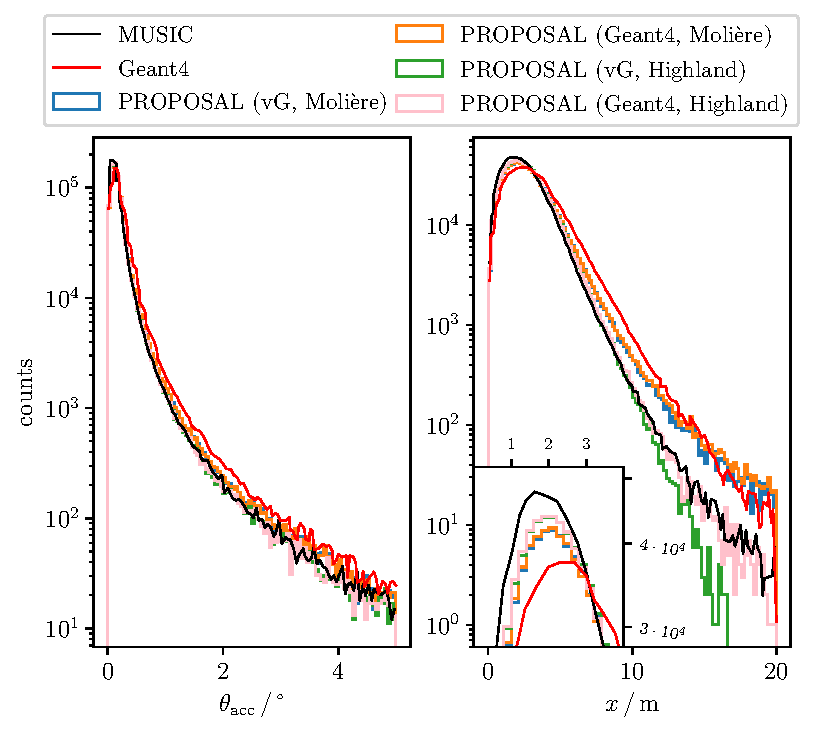
\includegraphics{../../deflection/plots/FINAL/2TeV_1e6events_accumulated_defl_paper_combined_zoom.pdf}
    \caption{A comparison of the results of MUSIC, Geant4 and PROPOSAL is presented for $\num{e6}$ muons propagated with 
    $E_{\text{i}} = \SI{2}{\tera\electronvolt}$ over a distance of 
    $\SI{3}{\kilo\meter}$ in water. A $v_{\mathrm{cut}} = \num{e-3}$ is set. In PROPOSAL, 
    bremsstrahlung and photonuclear interaction are parametrized either by 
    Van Ginneken (vG) or as in Geant4. Both scattering methods are checked. 
    Left: The accumulated deflection $\theta_{\mathrm{acc}}$ in degree is very similar in all cases.
    Right: The lateral displacement $x$ in meter depends 
    on the scattering method. Molière scattering leads to larger distances.
    In the zoomed-in figure, the region around the mode of the distributions are presented. 
    The mode of Geant4 is shifted to larger deflections.
    Detailed information are given in 
    Table~\ref{tab:compare_MUSIC}. The results for MUSIC and Geant4 are taken from 
    Ref.~\cite{comparison_MUSIC_GEANT4_2009}.}
    \label{fig:compare_MUSIC}
\end{figure*}
\begin{table*}
    \small
    \centering
    \caption{The survival probability $p_{\text{s}}$ that depends on the muon decay, the mean survived muon 
    energy $\overline{E}_{\text{f}}$, the mean scattered angle $\overline{\theta}$ 
    and the mean displacement $\overline{x}$ are presented for all cases from 
    Figure~\ref{fig:compare_MUSIC}. For all means, the standard deviation is given.
    The largest deflection and displacement is observed in the tool Geant4, which has the lowest mean survived energy. The lower the energy, the larger the deflection.}
    \begin{tabular}{l|cc|cccc}
        \toprule
        & MUSIC & Geant4 & \multicolumn{4}{c}{PROPOSAL} \\
        &  & & \multicolumn{2}{c}{Molière} & \multicolumn{2}{c}{Highland} \\
        &  &  & vG & Geant4 & vG & Geant4 \\
        \midrule
        $p_{\text{s}}\,/\,\si{\percent}$ & 77.9 & 79.3 &  \multicolumn{4}{c}{77.9}\\
        $\overline{E}_{\text{f}}\,/\,\si{\giga\electronvolt}$ & 323 & 317 & \multicolumn{4}{c}{331$\pm$178} \\
        $\overline{\theta}\,/\,\si{\degree}$ & 0.22 & 0.27 & 0.24$\pm$0.45 & 0.24$\pm$0.45 & 0.22$\pm$0.35 & 0.22$\pm$0.35   \\
        $\overline{x}\,/\,\si{\meter}$ & 2.6 & 3.3 & 2.9$\pm$2.6 & 2.9$\pm$2.6 & 2.7$\pm$1.6 & 2.7$\pm$1.7  \\
     \bottomrule
    \end{tabular}
    \label{tab:compare_MUSIC}
\end{table*}

In the following, two comparisons are performed with measured data for 
different energies and media.
A measurement of muon deflections in low-$Z$ materials was done by Attwood et al. \cite{attwood_2006}. 
From this it can be seen that for $Z < 4$ the scattering angle is overestimated 
by Molière scattering in Geant4. Hence, the lower scattering in PROPOSAL leads 
to a better precision especially in the region of outliers. The comparison is 
done in liquid $\text{H}_2$ with a thickness of $\SI{109}{\milli\meter}$ and an 
initial particle energy of $E_{\mathrm{i}} = \SI{199}{\mega\electronvolt}$, which 
results via the energy-momentum relation of an in Ref.~\cite{attwood_2006} used beam momentum 
of $p = \SI[per-mode=symbol]{168.9}{\mega\electronvolt\per\clight}$. 
In PROPOSAL, the simulations are done with two different energy cuts $v_{\mathrm{cut}} = \num{e-3}$ and $v_{\mathrm{cut}} = \num{e-5}$, 
but there is no significant difference between the resulting deflections.
The comparison is presented in Figure~\ref{fig:attwood_comparison}.

\begin{figure*}
    \centering 
    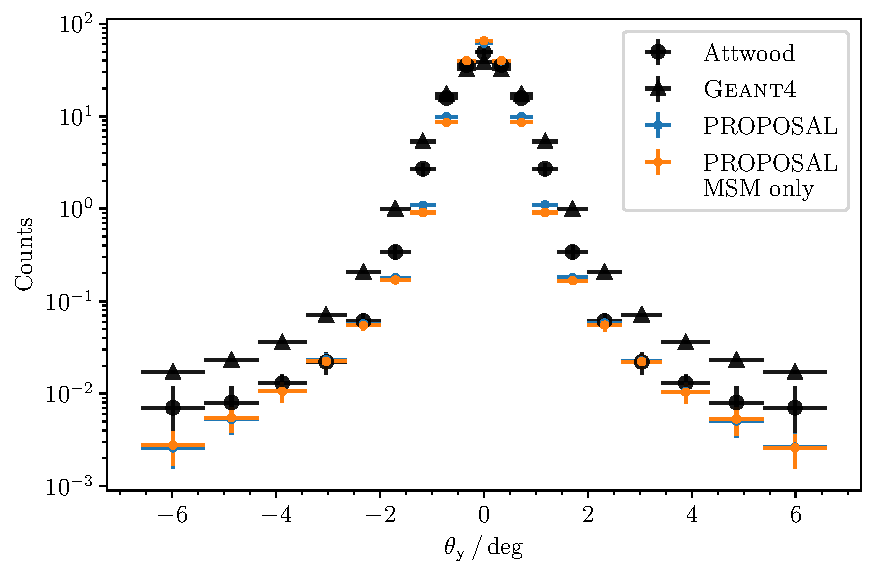
\includegraphics{../../deflection/plots/FINAL/attwood_comparison_moliere_199MeV_final_multi_mean_deg.pdf}
    \caption{
    Muons are 
    propagated with $E_{\mathrm{i}} = \SI{199}{\mega\electronvolt}$ through 
    $\SI{109}{\milli\meter}$ of liquid $\text{H}_2$.
    Measured data of Attwood et al. and simulation data of Geant4 are taken from Ref.~\cite{attwood_2006}.    
    The figure presents 
    the normalized counts in dependence of the projected scattering angle $\theta_{\mathrm{y}}$ in degree.
    In PROPOSAL, $100$ simulations each with $\num{e5}$ muons are performed for two different settings using the energy cut 
    $v_{\mathrm{cut}} = \num{e-5}$. The blue points present the mean considering stochastic deflections and Molière scattering, the orange points
    present the mean taking into account only Molière scattering.   
    The uncertainties on the $x$--axis result due to the measured bin widths. The $y$--uncertainties are the standard deviations.   
    The deflections are  
    underestimated in PROPOSAL, except at $\theta_{\mathrm{y}} \approx \SI{0}{\degree}$. At deflections $\SI{2}{\degree} < \theta_{\mathrm{y}} < \SI{5}{\degree}$, 
    the result seems to be more accurate than Geant4's. The consideration of the stochastic deflections shows no significant influence.}
    \label{fig:attwood_comparison}
\end{figure*}

The second measurement of muon deflections is done for higher energetic muons 
of $p = \SI[per-mode=symbol]{7.3}{\giga\electronvolt\per\clight}$ by Akimenko et al. \cite{akimenko_1984}.
In total, $\num{31125}$ muons are propagated through a $\SI{1.44}{\centi\meter}$ thick 
copper layer. Again, the two energy cuts mentioned before and the effect of stochastic deflections 
in comparison with Molière scattering only are checked. 
Neither between the two energy cuts, nor when using the stochastic deflection a significant difference occurs. 
PROPOSAL overestimates the angles for larger deflections. This observation differs from the comparison with Attwood, 
in which higher deflections are underestimated. In general, the higher muon energy 
leads to smaller deflections. The result is presented in Figure~\ref{fig:akimenko_comparison}.
\begin{figure*}
    \centering 
    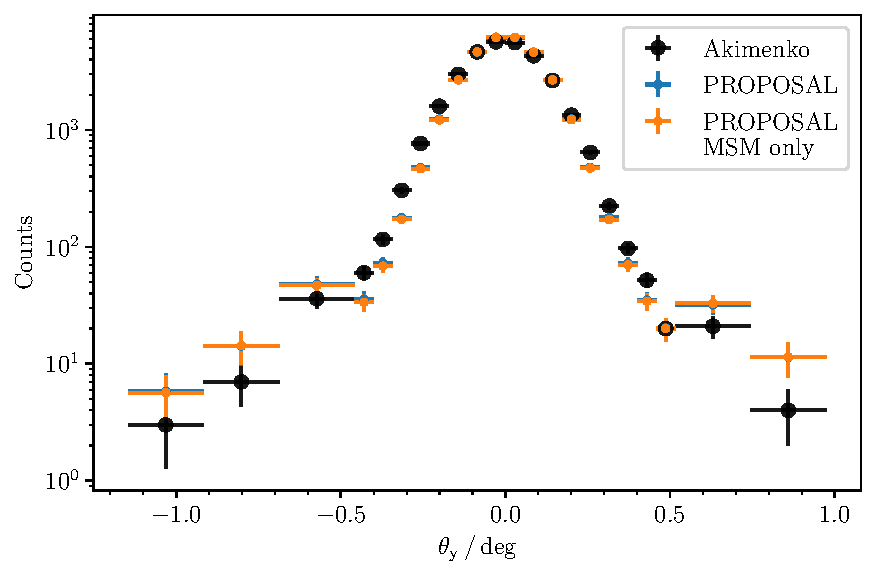
\includegraphics{../../deflection/plots/FINAL/akimenko_comparison_moliere_E7301MeV_final_multi_mean_deg.pdf}
    \caption{A comparison between two PROPOSAL settings and measured data by Akimenko et al. \cite{akimenko_1984} 
    is presented. $\num{100}$ simulations each with $\num{31125}$ muons with 
    $E_{\mathrm{i}} = \SI{7.301}{\giga\electronvolt}$ are propagated through a $\SI{1.44}{\centi\meter}$ 
    copper layer. The blue points present the mean considering stochastic deflections and Molière scattering, the orange points
    present the mean taking into account only Molière scattering. The uncertainties on the $x$--axis result due to the measured bin widths. The $y$--uncertainties are the standard deviations for PROPOSAL and the Poisson errors with $\sqrt{N}$ for Attwood, with $N$ as number of counts. Larger deflections are overestimated by PROPOSAL.
    Considering stochastic deflections has no significant impact.}
    \label{fig:akimenko_comparison}
\end{figure*}

For neutrino source searches based on entering muons, it is important to study the impact of the muon 
deflection on the angular resolution to estimate whether or not this needs to be 
taken into account as an additional source of uncertainty.
For this purpose, four different initial energies 
from $E_{\text{i}} = \SI{10}{\tera\electronvolt}$ to 
$E_{\text{i}} = \SI{10}{\peta\electronvolt}$ are used and the final 
energy is set to $E_{\text{f,\,min}} \geq \SI{10}{\giga\electronvolt}$ with 
$E_{\text{f,\,min}} < E_{\text{i}}$ for each simulation. 
In total $\num{36}$ simulations are performed. 
To compare the results of these simulations, the medians of the deflection distributions 
with a $\SI{95}{\percent}$ central interval are presented in 
Figure~\ref{fig:fit_median}.
The lower the final muon energy, the larger the accumulated deflection. 
For energies $E_{\text{f}} = \SI{1}{\peta\electronvolt}$, the median deflection 
is $\SI{e-4}{\degree}$. For energies $E_{\text{f}} = \SI{10}{\giga\electronvolt}$, 
angles larger than $\SI{1}{\degree}$ are possible. For energies  
$E_{\text{f}} \approx \SI{100}{\giga\electronvolt}$, 
there is a small overlap of the deflection with the angular resolution of KM3NeT 
\cite{KM3NeT_Resolution2021, KM3NeT_Resolution2016}. The resolution of IceCube is a bit worse and 
therefore not affected \cite{IceCube_Resolution2021}. 
The kinematic scattering angle between the incident neutrino and the produced muon is 
larger than the deflection in the presented region from $\SI{300}{\giga\electronvolt}$
to $\SI{200}{\tera\electronvolt}$. Here it must be noted that the kinematic angle 
and the resolution of ARCA (part of KM3NeT dedicated to search for very high-energetic neutrinos) are presented in dependence of the neutrino energy 
in Ref.~\cite{KM3NeT_Resolution2021, KM3NeT_Resolution2016}. Hence, a rescaling to the muon energy is applied using the average energy transfer of the neutrino to 
the nucleus \cite{GANDHI199681}. This shifts both curves to lower energies. 
Since all of these simulations are done 
in ice, the same simulations are done in water to compare the results for 
water-based experiments. The deviations of the medians
are less than $\SI{1}{\percent}$ for all energies.

Note that the distribution of deflection angles at a given final energy $E_{\mathrm{f}}$ in Figure~\ref{fig:fit_median} overlap for differing initial energies. This result indicates that the total deflection of a muon 
primarily depends on the final muon energy.
The initial muon energy is nearly irrelevant. 
Hence, the reconstructed muon 
energy in a detector can be used to estimate the deflection. For this 
purpose, a polynomial of degree three as 
\begin{equation}
     f(x) = a \cdot x^3 + b \cdot x^2 + c \cdot x + d \,,
    \label{eqn:fit_median}
\end{equation} 
can be used with the parameters 
\begin{align*}
    a =& +0.024 \pm 0.001\,,  & c =& +0.379 \pm 0.057\,,\\
    b =& -0.312 \pm 0.016\,,  & d =& -0.216 \pm 0.058\,,
\end{align*}
in the logarithmic space via 
\begin{align}
    g(x) =& 10^{f(x)}\,, & x =& \log_{10}\left(\frac{E_{\text{f}}}{\si{\giga\electronvolt}}\right)\,.
\end{align}
In general, the function $f(x)$ in Eq.~\eqref{eqn:fit_median} describes the median 
deflection of a muon after a propagated distance in ice for a given, respectively measured energy 
to estimate the deflection before the detector entry.

\begin{figure*}
    \centering 
    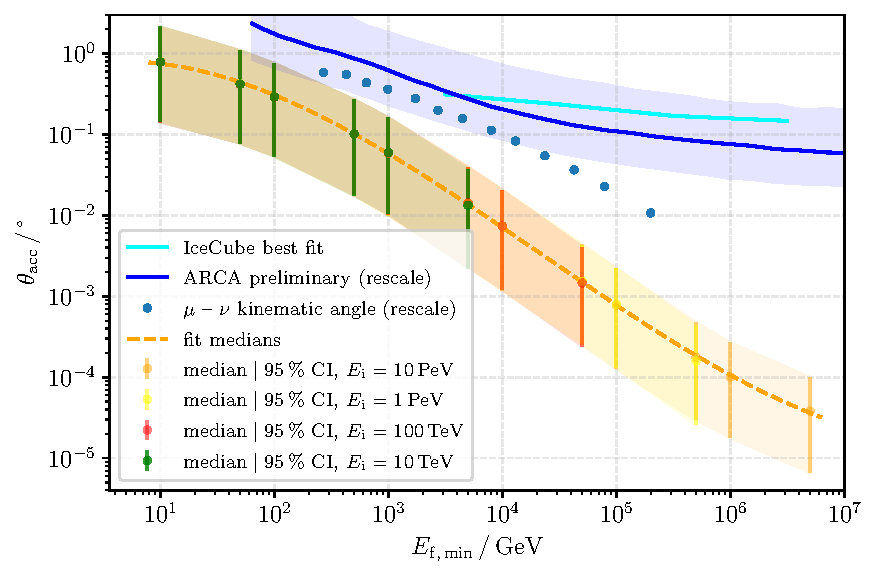
\includegraphics{../../deflection/plots/FINAL/fit_median_defl_cut_10percent_only_poly_new_resolution_rescale_no_icecube_paper_final.pdf}
    \caption{The median of the accumulated deflection $\theta_{\text{acc}}$ in degree 
    with a $\SI{95}{\percent}$ 
    central interval is shown for four different initial energies $E_{\text{i}}$. 
    Each data set includes more than $\num{50000}$ events with the requirement 
    that the true final particle energy $E_{\text{f}}$ is at most 
    $\SI{10}{\percent}$ below the set final energy $E_{\text{f,\,min}}$,   
    $E_{\text{f}} > E_{\text{f,\,min}} \cdot 0.9$. The energy cuts are $e_{\mathrm{cut}} = \SI{500}{\mega\electronvolt}$ and $v_{\mathrm{cut}} = 0.05$ and 
    Molière scattering is chosen. Simulations are performed in ice, the deviations 
    of the medians in a water-based simulation are smaller than $\SI{1}{\percent}$.
    Since the medians overlap for different initial energies, there is no 
    strong impact of the initial energy on the median deflection. These 
    medians can be fit by a third degree polynomial in the log-space as 
    shown in Eq.~\eqref{eqn:fit_median}. The kinematic angle between the muon and 
    neutrino is taken from Ref.~\cite{KM3NeT_Resolution2016}. Since the kinematic angle and 
    the angular resolution of ARCA (part of KM3NeT designed for high-energetic neutrino searches) taken from Ref.~\cite{KM3NeT_Resolution2021, KM3NeT_Resolution2016} are 
    presented in dependence of the neutrino energy, a rescaling to the muon energy is performed 
    using the average energy transfer to the nucleus \cite{GANDHI199681}. 
    For energies 
    $E_{\text{f}} \approx \SI{100}{\giga\electronvolt}$, there is a minimal influence of deflection on the angular resolution of 
    KM3NeT \cite{KM3NeT_Resolution2021}. The resolution shown by IceCube is not 
    impacted \cite{IceCube_Resolution2021}.}
    \label{fig:fit_median}
\end{figure*}

\section{Conclusion}\label{sec:conclusion}

Stochastic deflection, recently implemented in PROPOSAL 7.3.0, is 
used to study the muon deflection per interaction. The deflection 
is dominated by multiple scattering except for a few stochastic 
outliers by bremsstrahlung. These angles are lower than
$\sim\SI{1}{\degree}$. 

The results of PROPOSAL are compared with the common tools MUSIC and 
Geant4 and they are in good agreement. In low-$Z$ materials, the region of outlier 
deflections fits the measured data better with PROPOSAL, than Geant4. 
A second data comparison points out that PROPOSAL overestimates 
larger deflections at higher muon energies and underestimates at lower 
energies.

The median accumulated deflection depends primarily on the final muon energy, which can be interpreted as the muon energy at detector entry 
in neutrino telescopes or other muon detectors.
The outcome is fit by a polynomial and can be used for 
a theoretical estimation of the muon deflection in water and ice.
Since the result can be interpreted as the deflection before the detector entry, it defines a lower limit on the directional resolution.
At energies of $\SI{100}{\giga\electronvolt}$, there is potentially a small impact of the muon deflection on the angular 
resolution of KM3NeT.


\begin{acknowledgement}
  We acknowledge the funding by the Collaborative Research Center SFB $876$, SFB $1491$ 
  and the Deutsche Forschungsgemeinschaft by the project SA~$3867/$2-1.
\end{acknowledgement}


\printbibliography


\end{document}

